\item \textbf{Begin by using your knowledge of ARIMA (or SARIMA) modeling to conduct a univariate time series analysis and prediction of the NY Stock Exchange. Explain your process, present your chosen model, examine the residuals, and evaluate its performance as follows:} 
\begin{enumerate}
\item \textbf{Hold out the last 3 months of 2017 for out-of-sample prediction. Plot the predictions and confidence intervals and report the forecasting error using appropriate metrics.}
\item \textbf{Use a rolling window approach, with a training window of 3 years and daily increments, predict the next day. Again, plot the predictions and confidence intervals and report the forecasting error using appropriate metrics.}
\end{enumerate}






\textit{ The general process for \gls{arima} model is the following:}
\begin{enumerate}
\item \textit{Visualize the Time Series Data (Figure
        \ref{fig:Ass2_Q2_raw_signal})}
\item \textit{Transform and make the time series data stationary (Figure
        \ref{fig:Ass2_Q2_1diff_signal})}
\item \textit{Plot the \gls{ACF} and \gls{PACF} (Figure
        \ref{fig:Ass2_Q2_PACF_ACF_1diff})}
\item \textit{Construct the \gls{arima} Model or Seasonal \gls{arima} based on the data }
\item \textit{Identify optimal model based on Information Criteria, like \gls{AIC} }
\item \textit{Evaluate the residuals using statistical test, \gls{ACF}, \gls{PACF}, etc. (Figure
         \ref{fig:Ass2_Q2_best_model_residual})}
\item \textit{Use the model to make predictions (Figure
        \ref{fig:Ass2_Q2_Automatic_model_forcasting})}
\item \textit{Calculate forecasting error}


\end{enumerate}


\begin{figure}[H]
    \centering
    \begin{minipage}[b]{1\textwidth}
        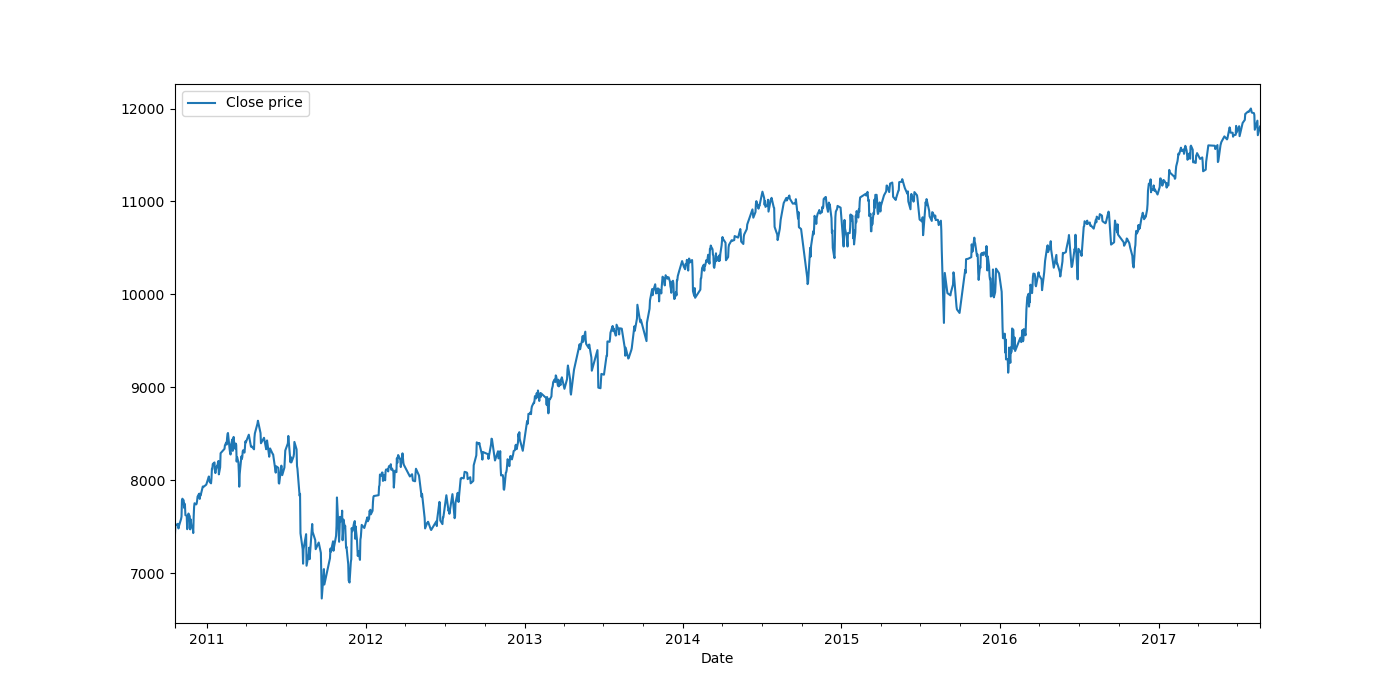
\includegraphics[width=\textwidth]{figures/Ass2/Ass2_Q2_raw_signal.png}
    \end{minipage}
    \caption{The raw signal of the dataset.}
    \label{fig:Ass2_Q2_raw_signal}
\end{figure}

\begin{figure}[H]
    \centering
    \begin{minipage}[b]{1\textwidth}
        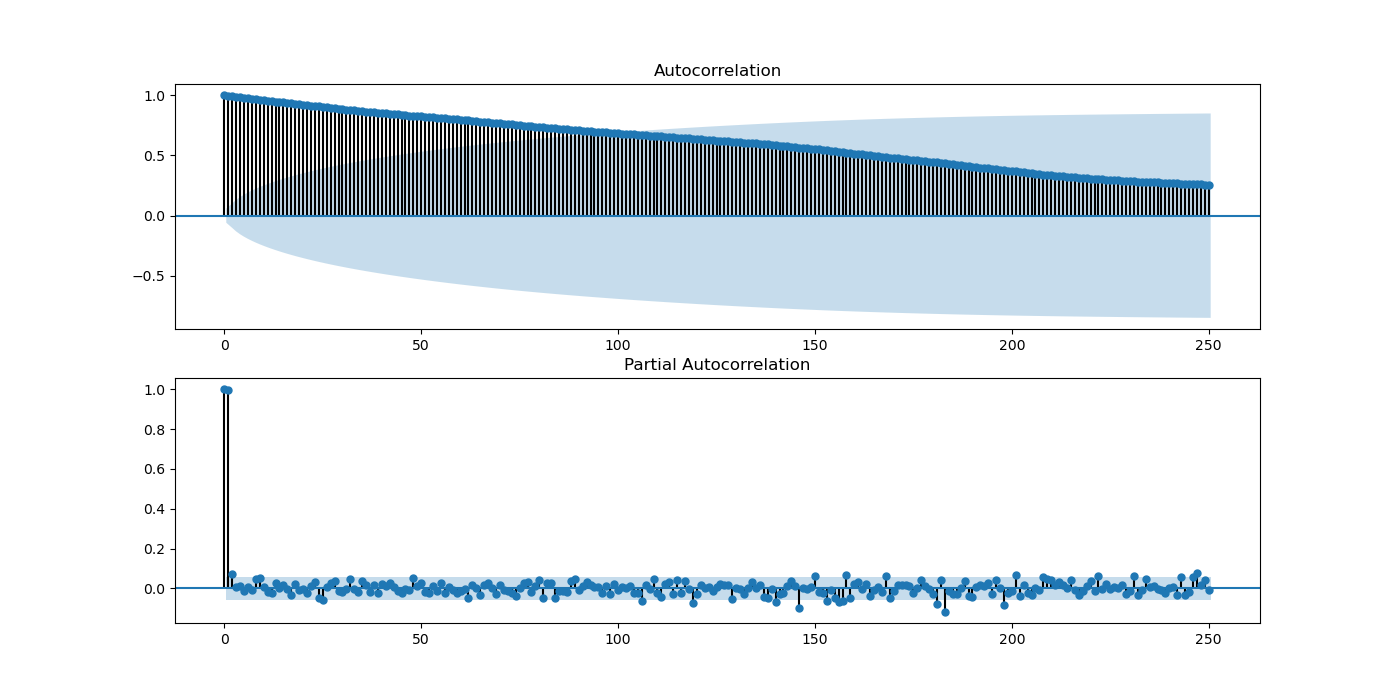
\includegraphics[width=\textwidth]{figures/Ass2/Ass2_Q2_PACF_ACF.png}
    \end{minipage}
    \caption{A plot of \gls{ACF} and \gls{PACF} of the dataset.}
    \label{fig:Ass2_Q2_PACF_ACF}
\end{figure}


\textit{Figures \ref{fig:Ass2_Q2_raw_signal} and \ref{fig:Ass2_Q2_PACF_ACF} indicate the raw signal along with its \gls{ACF} and \gls{PACF} plots. \gls{ACF} and \gls{PACF} plots allow us to determine how correlated points are with each other. Furthermore, the period of the seasonal component can be calculated by \gls{ACF}. As can be seen, \gls{ACF} plot has no oscillation, therefore there is no seasonal component related to the our time series.}




\textit{In order to turn the dataset to a stationary dataset, we used a first-order differencing. Table \ref{tab:Ass2_Q2_ADF_1diff} indicates the result of \gls{ADF}  on the first-order differencing. As this test shows, the data is a stationary data. Figures \ref{fig:Ass2_Q2_1diff_signal} and \ref{fig:Ass2_Q2_PACF_ACF_1diff} indicate the $1^{st}$ order differencing signal along with its \gls{ACF} and \gls{PACF} plots. These two plots also show that the data is stationary. }

\begin{table}[H]
\centering
\caption{The result of the \gls{ADF} on the $1^{st}$ order differencing in the dataset.}
\label{tab:Ass2_Q2_ADF_1diff}
\begin{tabular}{lr}
\toprule
{} &            0 \\
\midrule
ADF Statistic               &   -25.690334 \\
p-value                     &     0.000000 \\
\#Lags Used                  &     1.000000 \\
Number of Observations Used &  1111.000000 \\
Critical Value (1\%)         &    -3.436250 \\
Critical Value (5\%)         &    -2.864145 \\
Critical Value (10\%)        &    -2.568157 \\
\bottomrule
\end{tabular}

\end{table}

\begin{figure}[H]
    \centering
    \begin{minipage}[b]{1\textwidth}
        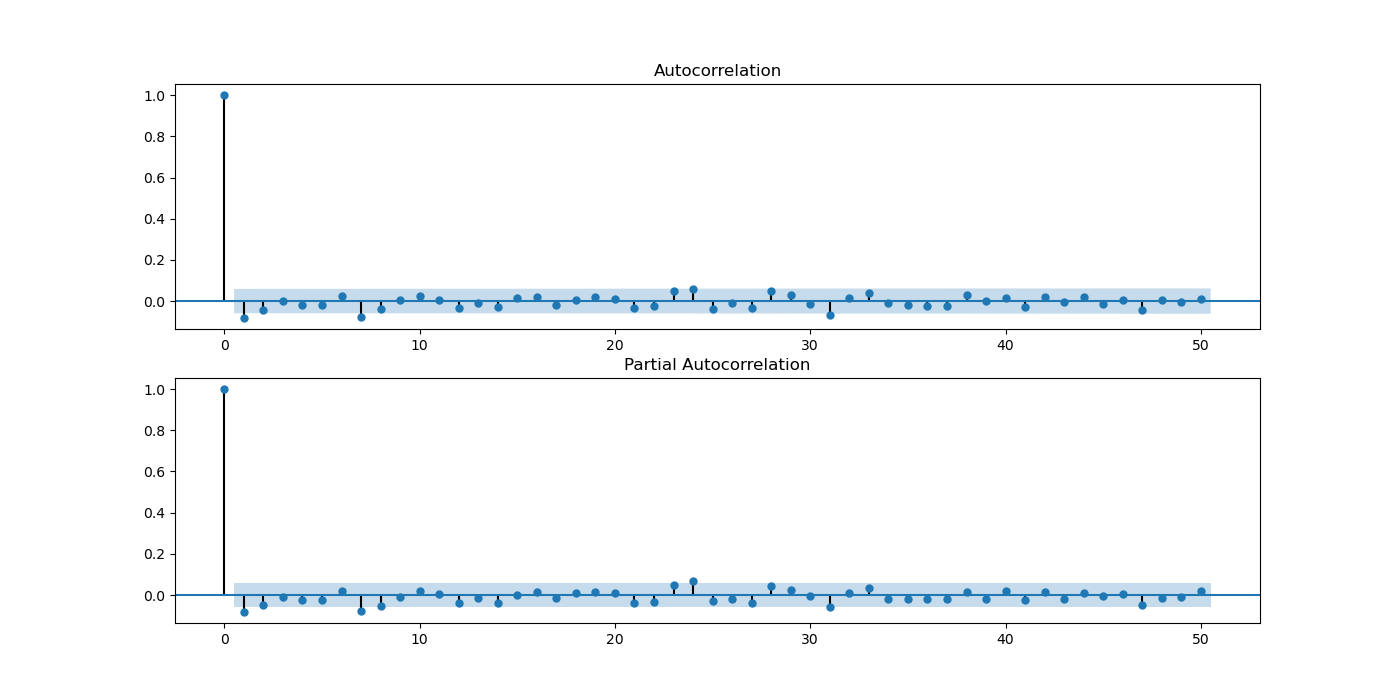
\includegraphics[width=\textwidth]{manuscript/src/figures/Ass2/Ass2_Q2_PACF_ACF_1diff.png}
    \end{minipage}
    \caption{ A plot of the \gls{ACF} and \gls{PACF} on the $1^{st}$ order differencing in the dataset.}
    \label{fig:Ass2_Q2_PACF_ACF_1diff}
\end{figure}
\begin{figure}[H]
    \centering
    \begin{minipage}[b]{1\textwidth}
        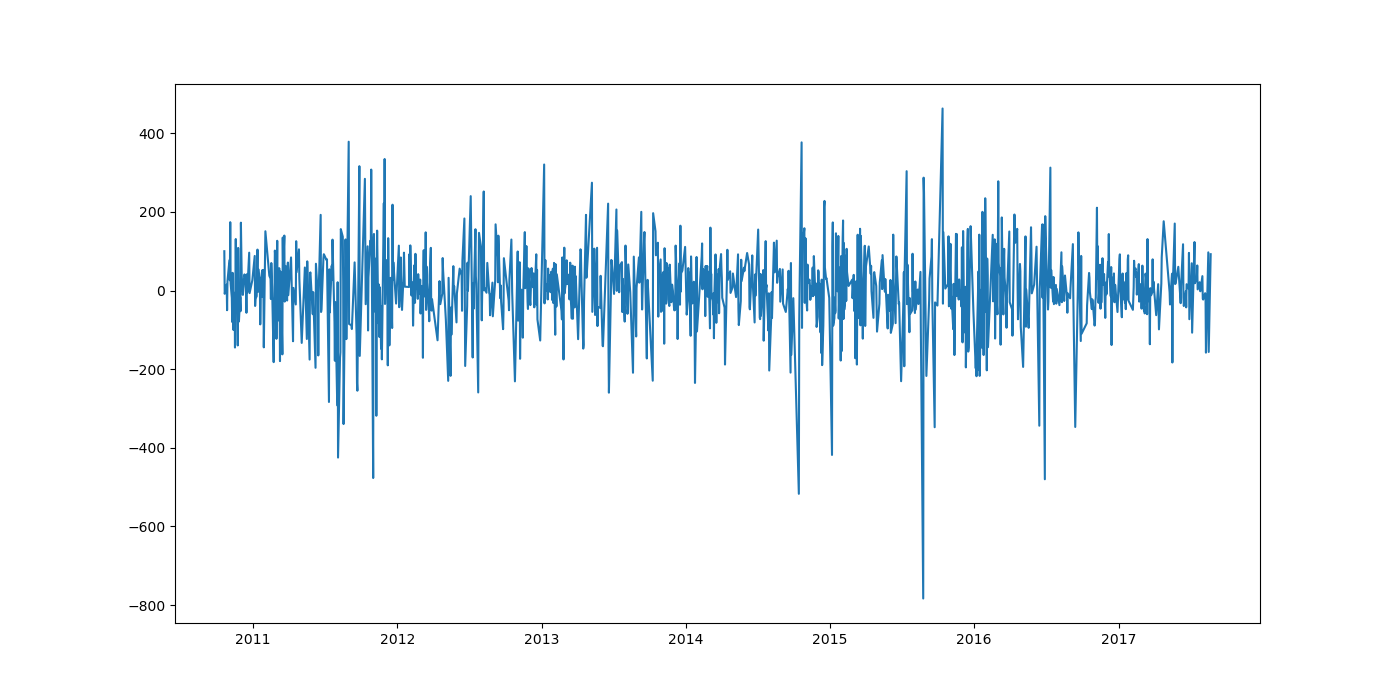
\includegraphics[width=\textwidth]{manuscript/src/figures/Ass2/Ass2_Q2_1diff_signal.png}
    \end{minipage}
    \caption{ The signal of $1^{st}$ order differencing.}
    \label{fig:Ass2_Q2_1diff_signal}
\end{figure}



\textit{We used grid search and interpreting \gls{ACF} and \gls{PACF} plots to select the best order for \gls{arima}.}

\textit{Since both \gls{ACF} and \gls{PACF} (see figure \ref{fig:Ass2_Q2_PACF_ACF_1diff}) have one significant lag, it can conclude that both AR order (q) and MA order (p) are one. Also, based on using $1^{st}$ order differencing, the integrated order (d) set 1.}

\textit{In grid search, we set a space search to find the model that had the lowest error. Table \ref{tab:ass2_Q2_1} shows our space search. This method selected the order \gls{arima}(1, 1, 1) as the best-fitted model.}

\begin{table}[H]
\centering
\caption{The space search of grid search.}
\label{tab:ass2_Q2_1}
\begin{tabular}{lcc}
\toprule
\# & hyper-parameter      & values\\ \hline
\midrule

1 & p & $1 \thicksim 4$               \\ \hline
2 & q & $1 \thicksim 4$               \\ \hline
3 & d & 1               \\ \hline
\bottomrule
\end{tabular}
\end{table}

\textit{Figure \ref{fig:Ass2_Q2_best_model_residual} indicates the residual of best-fitted model. As this plot illustrates, the residual signal of model has a Gaussian distribution with zero mean. In addition, the \gls{ACF} plot shows that this signal is a stationary signal.}



\begin{figure}[H]
    \centering
    \begin{minipage}[b]{1\textwidth}
        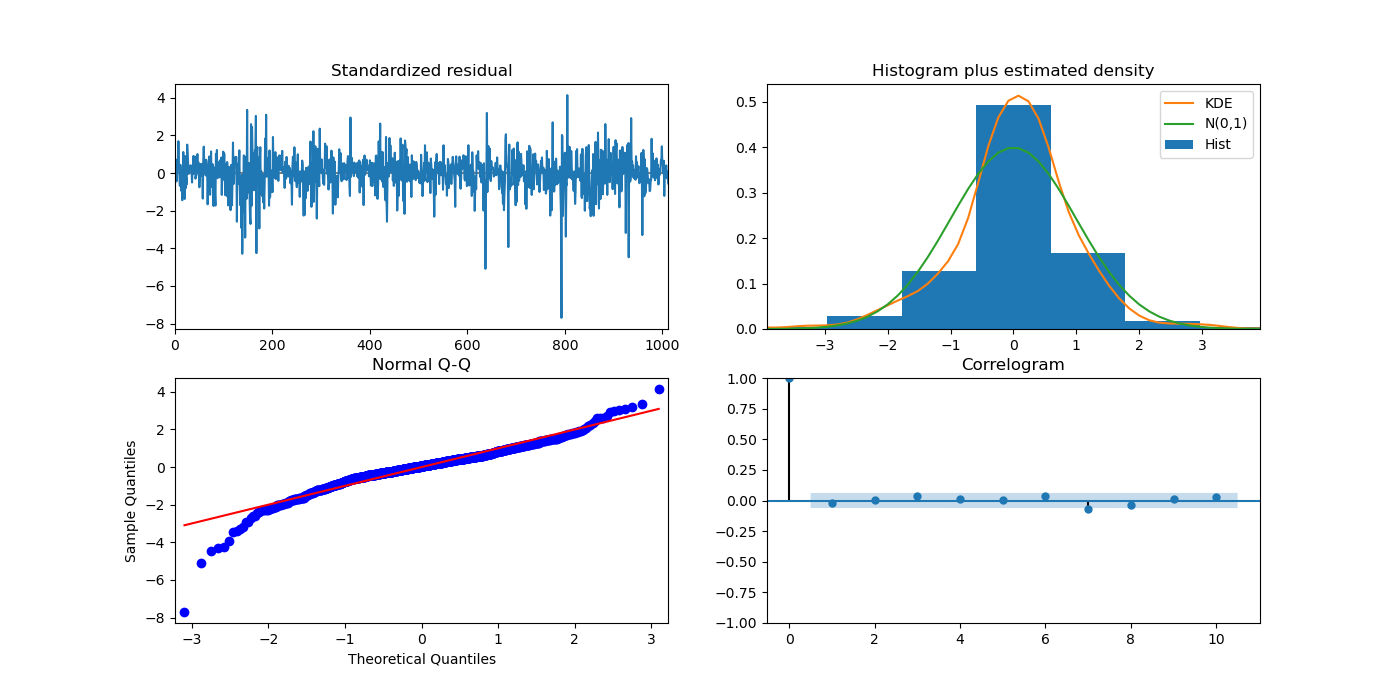
\includegraphics[width=\textwidth]{manuscript/src/figures/Ass2/Ass2_Q2_best_model_residual.png}
    \end{minipage}
    \caption{The residual  of the best-fitted model (\gls{arima}(1, 1, 1)) based on grid search.}
    \label{fig:Ass2_Q2_best_model_residual}
\end{figure}

  
\textit{To predict, we split data into test and train set. About 35 samples for test set and others for training. Figure \ref{fig:Ass2_Q2_Automatic_model_forcasting} demonstrates the output of the best-fitted model. As can be seen, the model could predict the upward trend. The obtained RMS error was 294.506.}

\begin{figure}[H]
    \centering
    \begin{minipage}[b]{1\textwidth}
        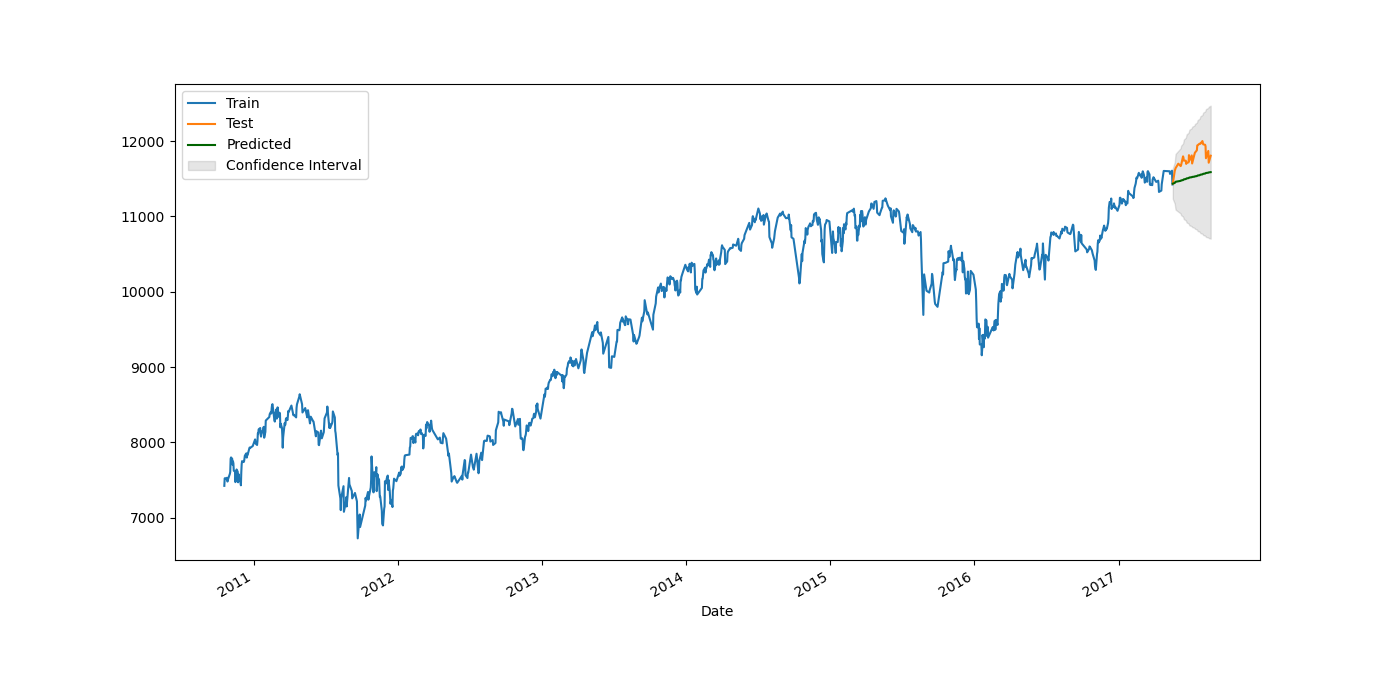
\includegraphics[width=\textwidth]{manuscript/src/figures/Ass2/Ass2_Q2_Automatic_model_forcasting.png}
    \end{minipage}
    \caption{The prediction and actual data of \gls{arima}(1, 1, 1) model.}
    \label{fig:Ass2_Q2_Automatic_model_forcasting}
\end{figure}


\textit{For the rolling window approach, we predicted only one day. Then the actual value of this day was added to the training set while our training set had a fixed size. We considered less than 500 samples (approximately three years).}

\textit{Since both the training data set did not change, we used the same order of the last part. Figures \ref{fig:Ass2_Q2_Rolling_Forecast} and \ref{fig:Ass2_Q2_Rolling_Forecast_1} demonstrate the output of the rolling window model. As can be seen, the model could follow the the test set. In addition, the RMS error was reduced from 294.506 to 69.371.}

\begin{figure}[H]
    \centering
    \begin{minipage}[b]{1\textwidth}
        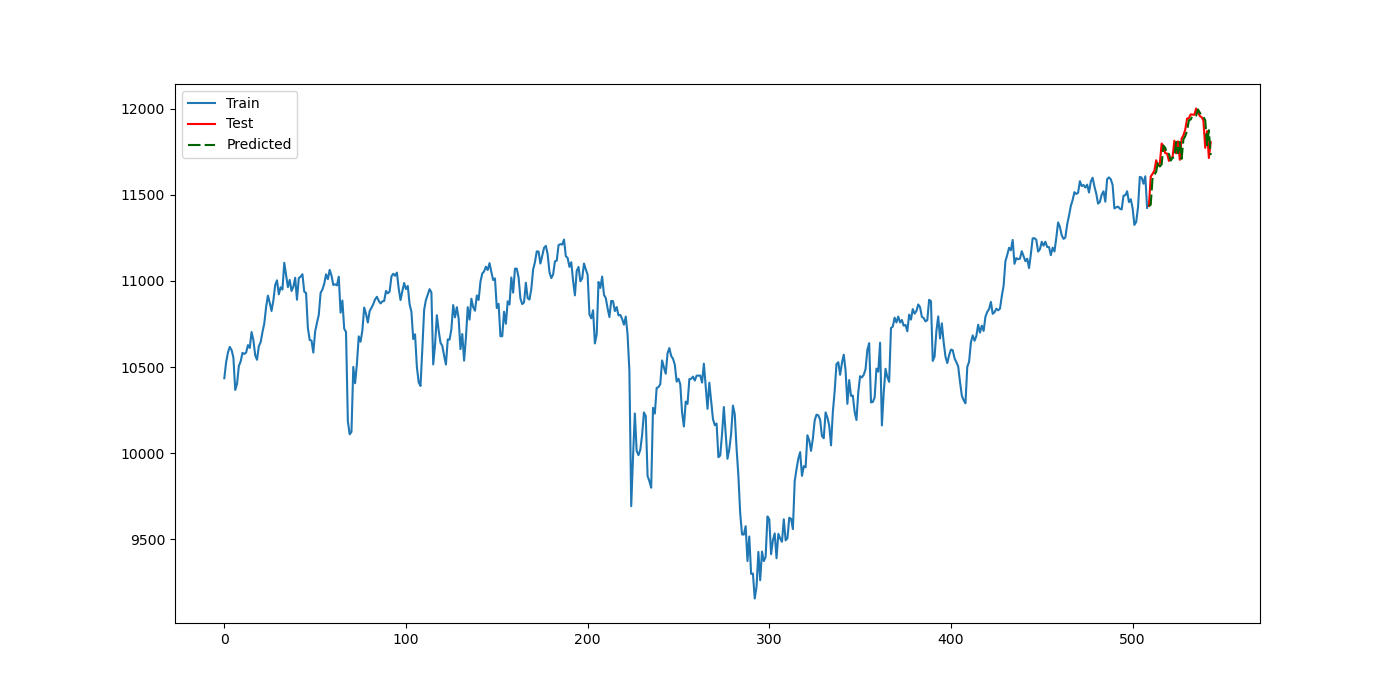
\includegraphics[width=\textwidth]{manuscript/src/figures/Ass2/Ass2_Q2_Rolling_Forecast_1.png}
    \end{minipage}
    \caption{The prediction and actual data of \gls{arima}(1, 1, 1) model in rolling windows approach.}
    \label{fig:Ass2_Q2_Rolling_Forecast_1}
\end{figure}

\begin{figure}[H]
    \centering
    \begin{minipage}[b]{1\textwidth}
        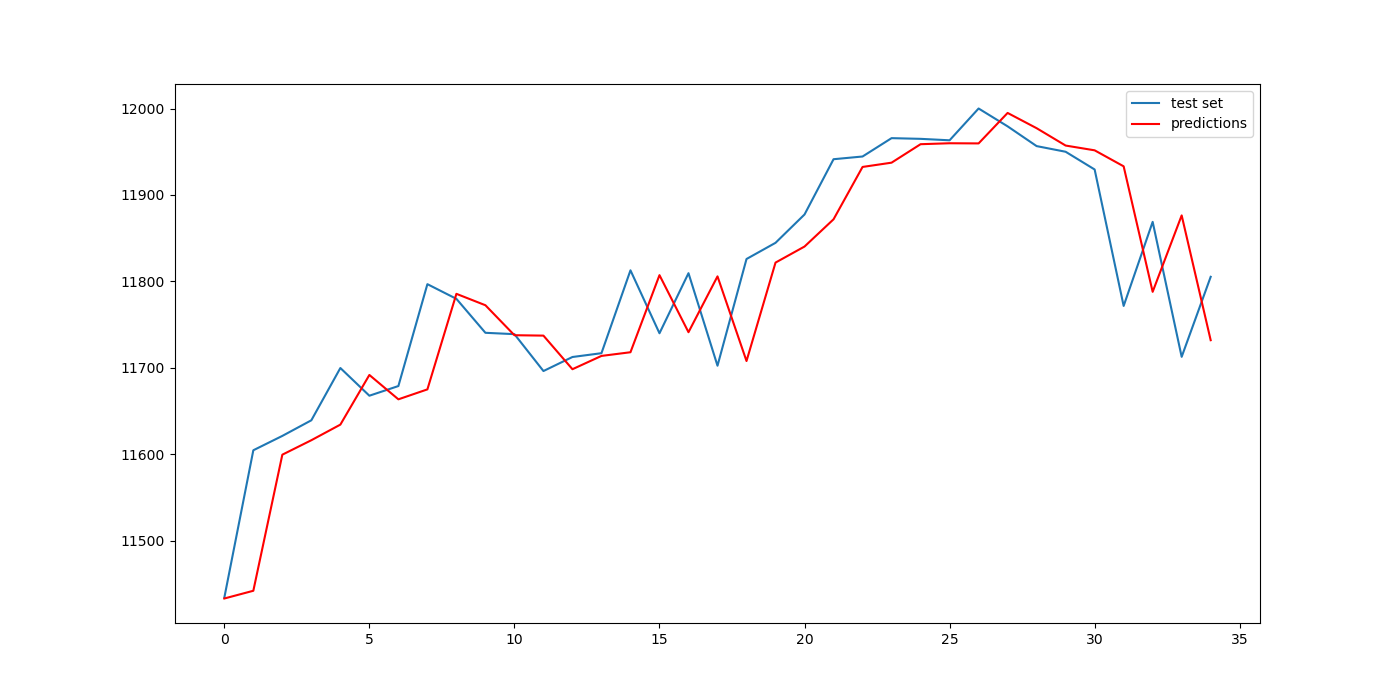
\includegraphics[width=\textwidth]{manuscript/src/figures/Ass2/Ass2_Q2_Rolling_Forecast.png}
    \end{minipage}
    \caption{The prediction and test set of \gls{arima}(1, 1, 1) model in rolling windows approach.}
    \label{fig:Ass2_Q2_Rolling_Forecast}
\end{figure}




